
\documentclass[t, 11pt]{beamer}
%\pdfmapfile{+sansmathaccent.map}
%%% Работа с русским языком
\usepackage{cmap}				
\usepackage{mathtext} 				
\usepackage[T2A]{fontenc}		
\usepackage[utf8]{inputenc}			
\usepackage[russian, english]{babel}	

\usetheme{Montpellier}
\usecolortheme{beaver} % Цветовая схема



%%% Работа с картинками
\usepackage{graphicx}

\usepackage{csquotes}

\hypersetup{				
	colorlinks=true,       	
	linkcolor=blue,          
	citecolor=black,       
	filecolor=magenta,      
	urlcolor=red           
}
%% табличка
\usepackage{booktabs, caption, makecell}
\usepackage{threeparttable}

%% график нормального распределения 
\usepackage{tikz}
\usepackage{xcolor}
\usepackage{pgfplots}
\pgfplotsset{compat=1.7}

%% доп символы
\usepackage{newunicodechar}

\newcommand\Warning{%
	\makebox[1.4em][c]{%
		\makebox[0pt][c]{\raisebox{.1em}{\small!}}%
		\makebox[0pt][c]{\color{red}\Large$\bigtriangleup$}}}%

%\newunicodechar{⚠}{\Warning}

\title {Regression properties}
\subtitle{what do we need know about}
\author{Chuvakin Sergey}
\date{\today}
\institute[<<Anthropology and Sociology major>>]{<<School of Advanced Studies>>}

\begin{document}

	
	\frame[plain]{\titlepage}		
	
	\section{Outline}
	
		\begin{frame} 
			\frametitle{\insertsection} 
			\begin{itemize}
				\item Significance
				\item Regression output (table)
				\item Regression plot
				\item Standart Error
				\item T-value
				\item P-value
				\item Confindence Intervals 
				\item R-squared 
			\end{itemize}
\end{frame}

\section{Significance}

		\begin{frame} 
	\frametitle{\insertsection} 
	Significance tells if we can make a proper, consistent and robust inference out of our data. 
\end{frame}	

\section{Regression line}
\begin{frame} 
	\frametitle{\insertsection} 
	\begin{center}
		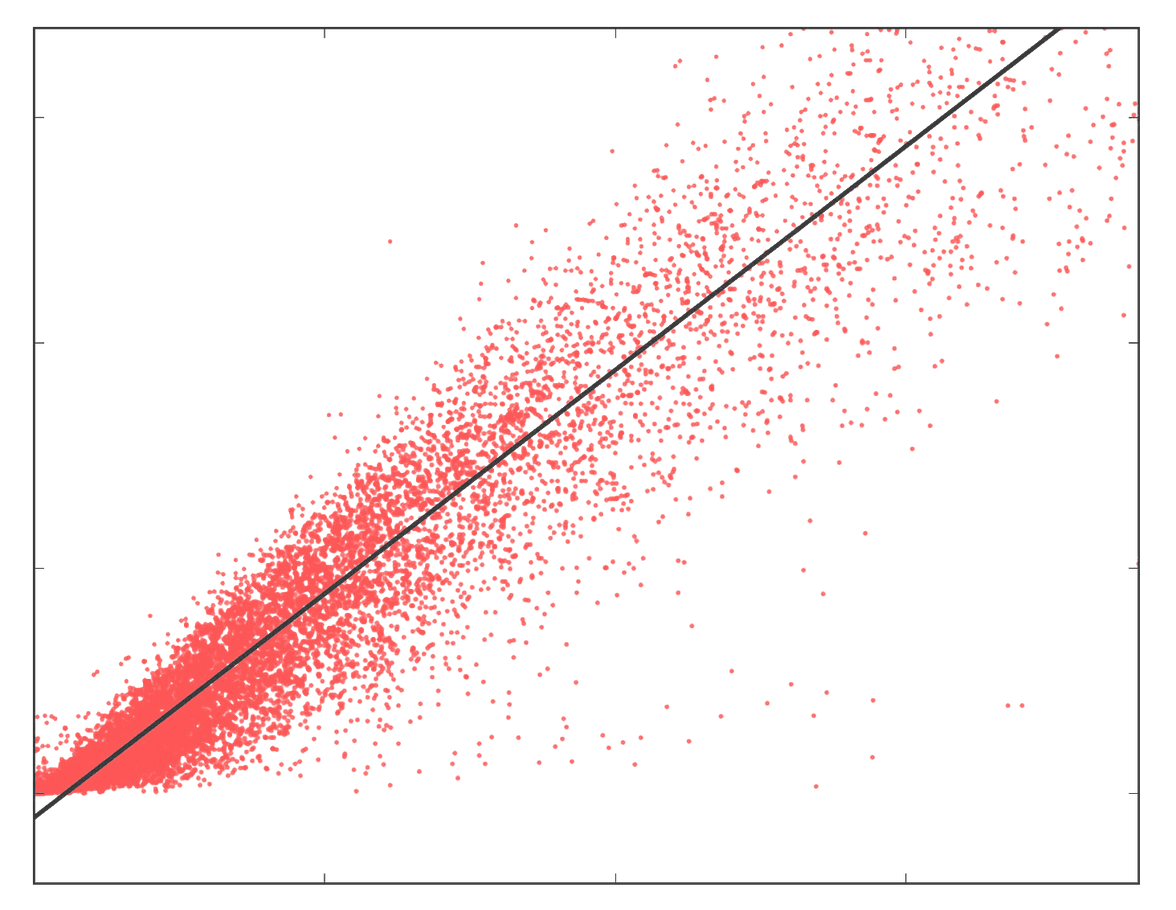
\includegraphics[scale=0.4]{reg_2d_line}
	\end{center}
\end{frame}	

\begin{frame} 
	\frametitle{\insertsection} 
	\begin{center}
		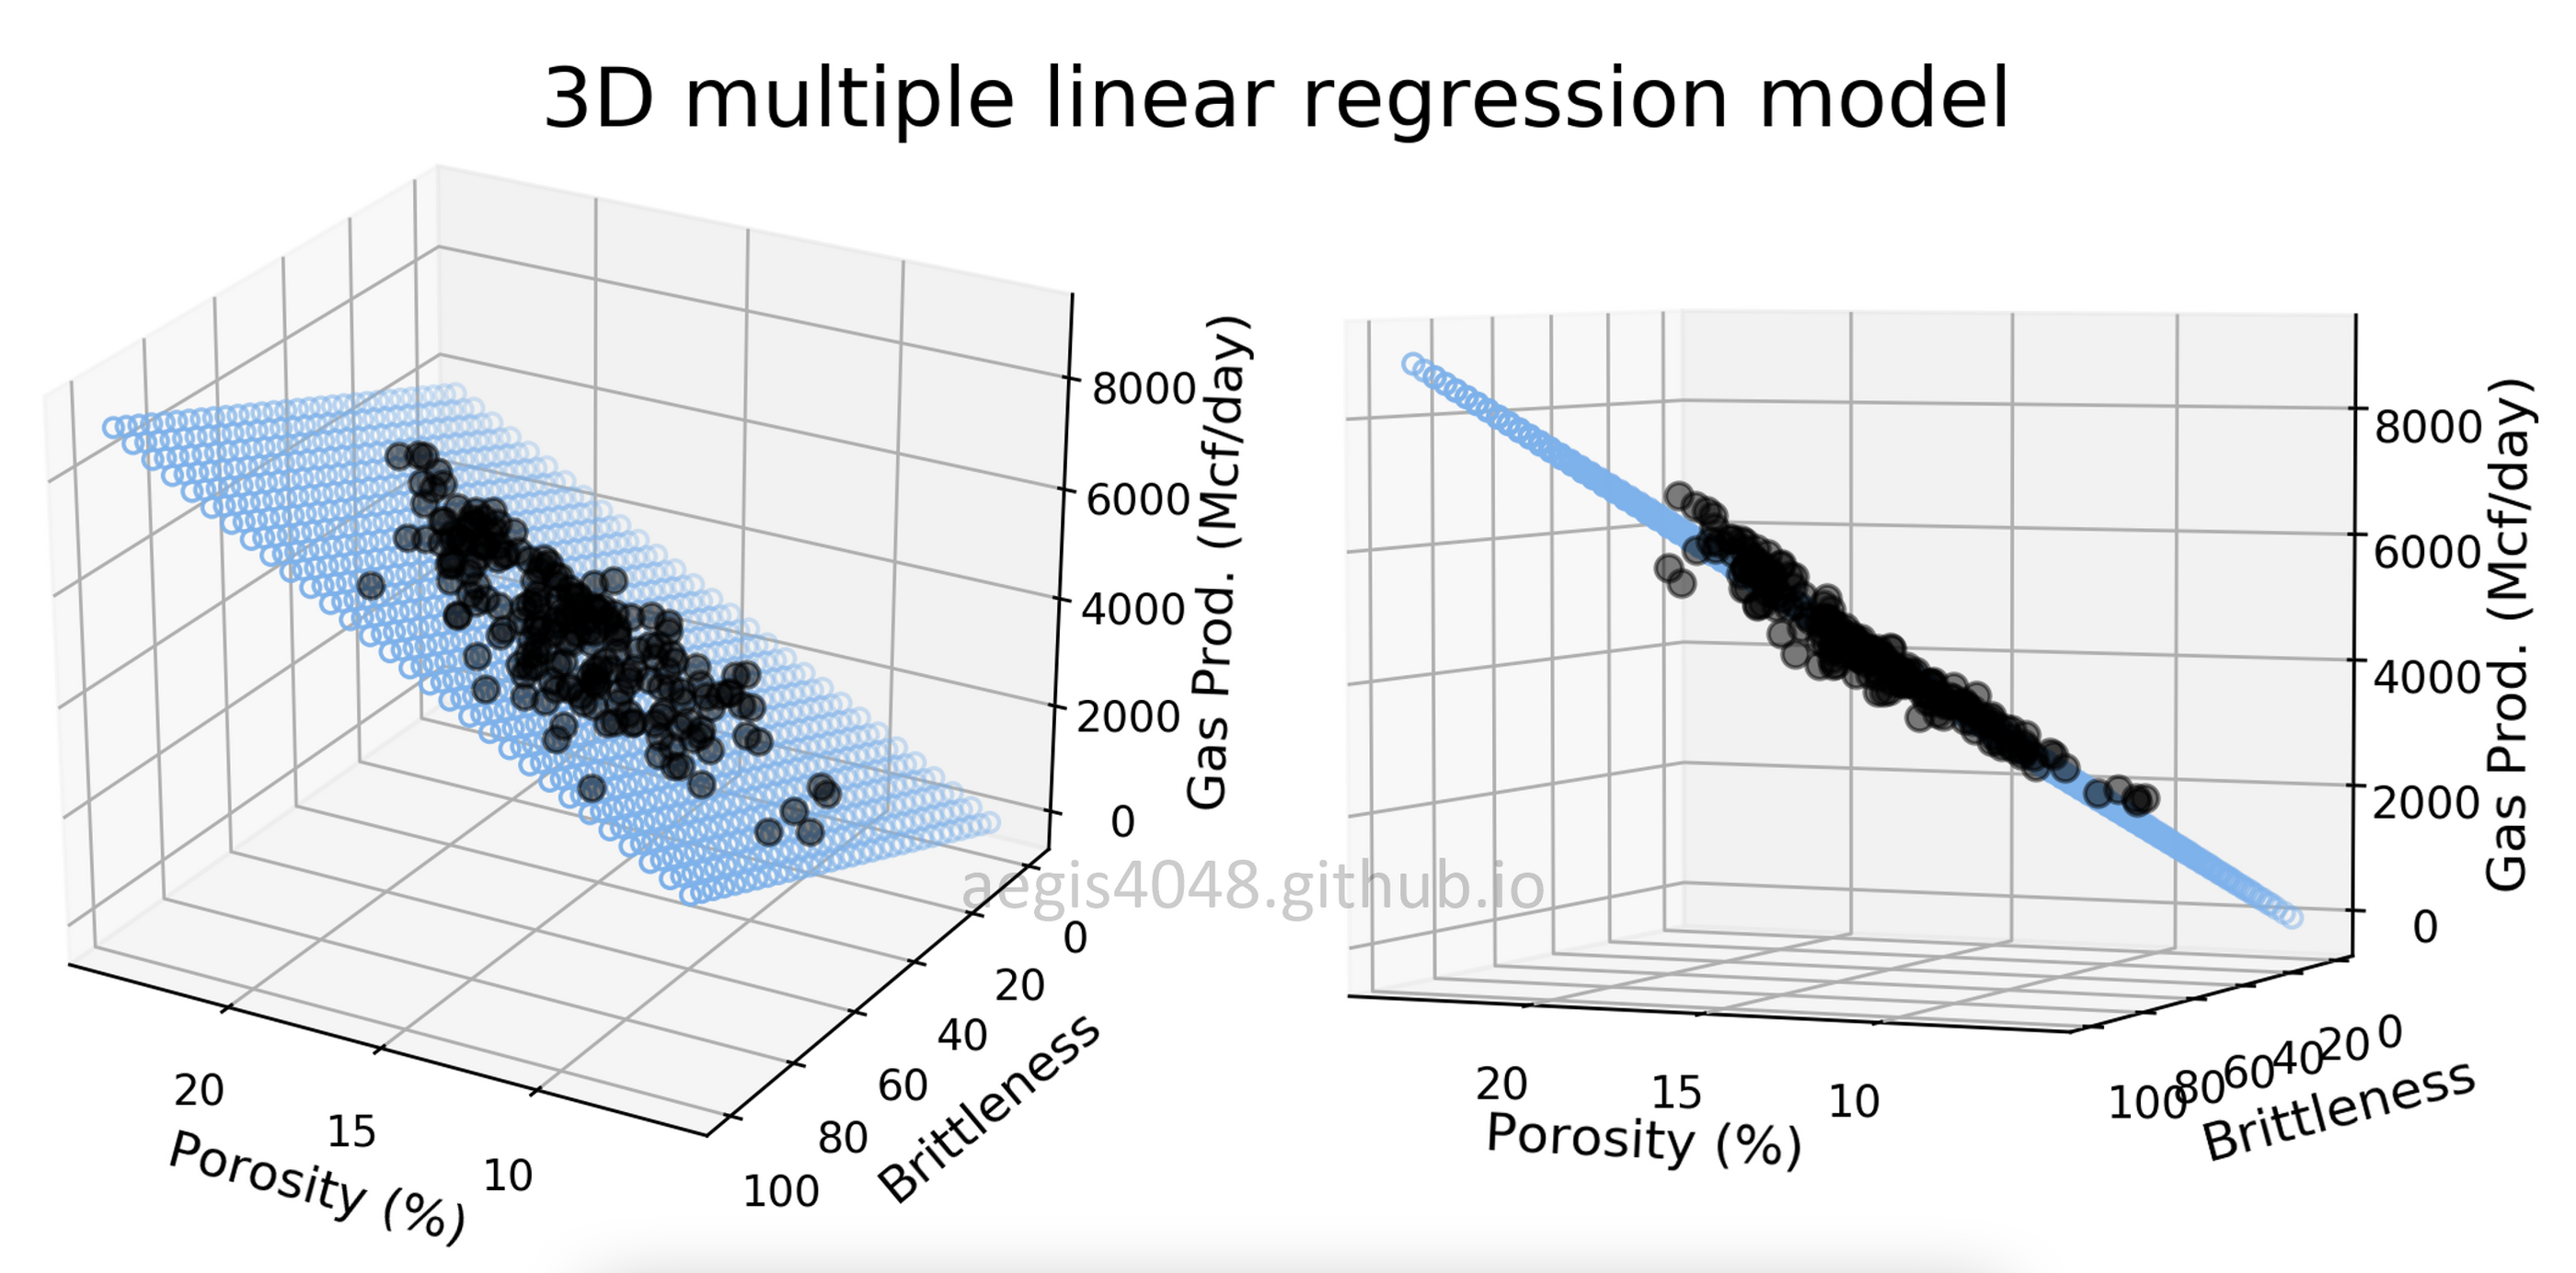
\includegraphics[scale=0.2]{reg_line_3d}
	\end{center}
\end{frame}	

\begin{frame} 
	\frametitle{\insertsection} 
	\begin{center}
		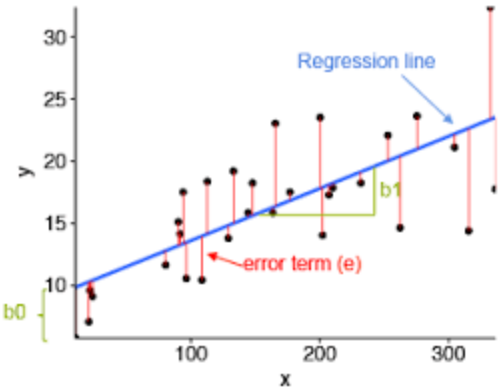
\includegraphics[scale=0.7]{reg_res_2d}
	\end{center}
\end{frame}	

\begin{frame} 
	\frametitle{\insertsection} 
	\begin{center}
		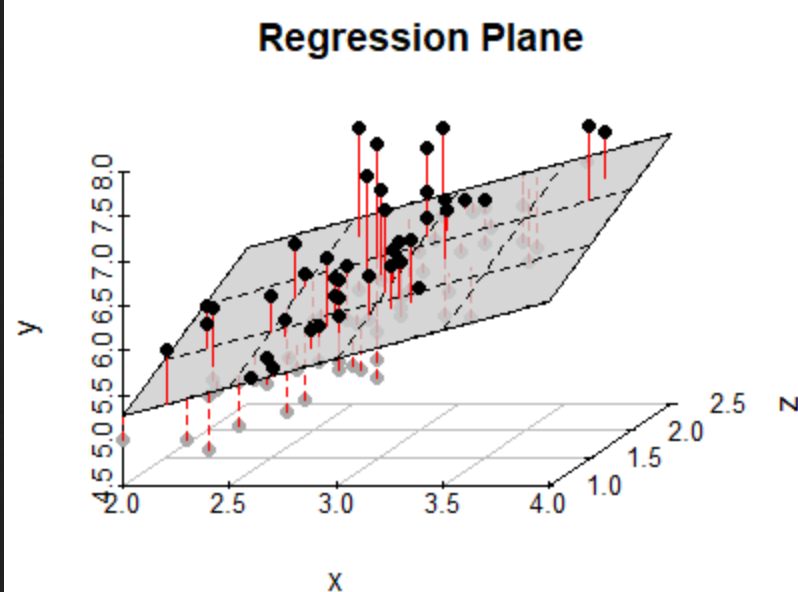
\includegraphics[scale=0.4]{reg_res_3d}
	\end{center}
\end{frame}	

\section{Regression output (table)}

	\begin{frame} 
	\frametitle{\insertsection} 
		\begin{center}
		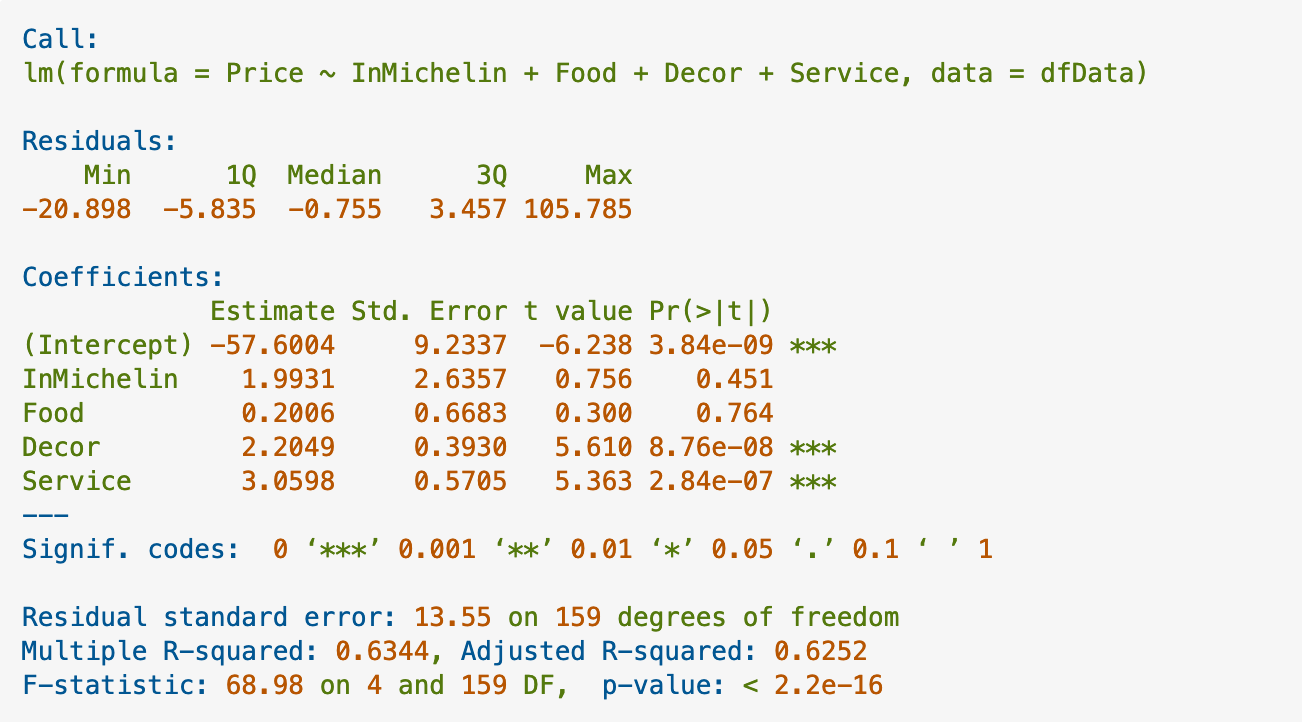
\includegraphics[scale=0.4]{reg_output_r}
	\end{center}
\end{frame}	

\section{Standart Error}

\begin{frame} 
	\frametitle{\insertsection} 
 SE - can be interpreted as standart deviation of beta coeficient. 
 
 $$se(\beta_i) = \frac{\hat{\sigma}}{\sqrt{\Sigma x_i^2}}$$
 
  $$\hat{\sigma} = \sqrt{ \frac{\Sigma \hat{u}_i^2}{n-2} }$$
  
  $$\hat{u}_i = \bar{y}_i - y_i$$

 
 
\end{frame}	


\begin{frame} 
	\frametitle{\insertsection} 

	\begin{itemize}
		\item x - predictor
		\item $\beta$ - coeficient
		\item u - Residual Sum of Squares 
		\item y - target
		\item $\bar{y}$ - predicted target
		\item n - number of degrees of freedom
	\end{itemize}
	
	
\end{frame}	

\section{Student's value}

\begin{frame} 
	\frametitle{\insertsection} 
	t- value - part of T-distribution that helps to uderstatnd if certain coeficient differs from 0. 
	
	$$t-value = \frac{\beta} {se(\beta)}$$
	
	What's next?
	
	\begin{enumerate}
		\item Find number of DF
		\item Guess level of significance you need
		\item Find treshhold in matrix \href{http://www.sthda.com/english/wiki/t-distribution-table}{here}
		\item If your t-value is higher that means that coef is significant
	\end{enumerate}

\end{frame}	

\section{P-value}
	\begin{frame} 
		\frametitle{\insertsection} 
	 	P - value - it's just convinient form of t-student value. 
		\begin{itemize}
			\item if P-value is below than 0.05 that means that we can reject null hypothesis (coef is signinfcant)
			\item if  P-value is above than 0.05 that means that we can not reject null hypothesis (coef is not  signinfcant)
			\end{itemize}
		
	\end{frame}	

\section{Confidence Intervals}

\begin{frame}
	\frametitle{\insertsection} 
	Confidence interval can be calculated even for $\beta$ coefs. 
	
	Steps to calculate:
	\begin{enumerate}
		\item Calculate Margin Error
		
		ME = treshhold of t-value * standard error
		
		\item Lower and Upper bounds: $ CI = \beta \pm ME$ 
		\end{enumerate}
	
\vspace{1cm}

If CI includes zero, this automatically means, that coef is not significant. The same aproach is applied to get Prediction Interval. Ypu need just change $\beta$ to $\hat{y}$. 
	
	\end{frame}

\section{Prediction Intervals}

\begin{frame}
	\frametitle{\insertsection} 
	The same aproach is applied to get Prediction Interval. Ypu need just change $\beta$ to $\hat{y}$. 
	
	$$\hat{y} \pm t \times \sqrt{ MSE \times (1 + \frac{1}{n} + \frac{(x_h- \bar{x})^2}{\Sigma (x_i- \bar{x})^2}) }$$
	
\end{frame}

\begin{frame}
	\frametitle{\insertsection} 
	\begin{center}
		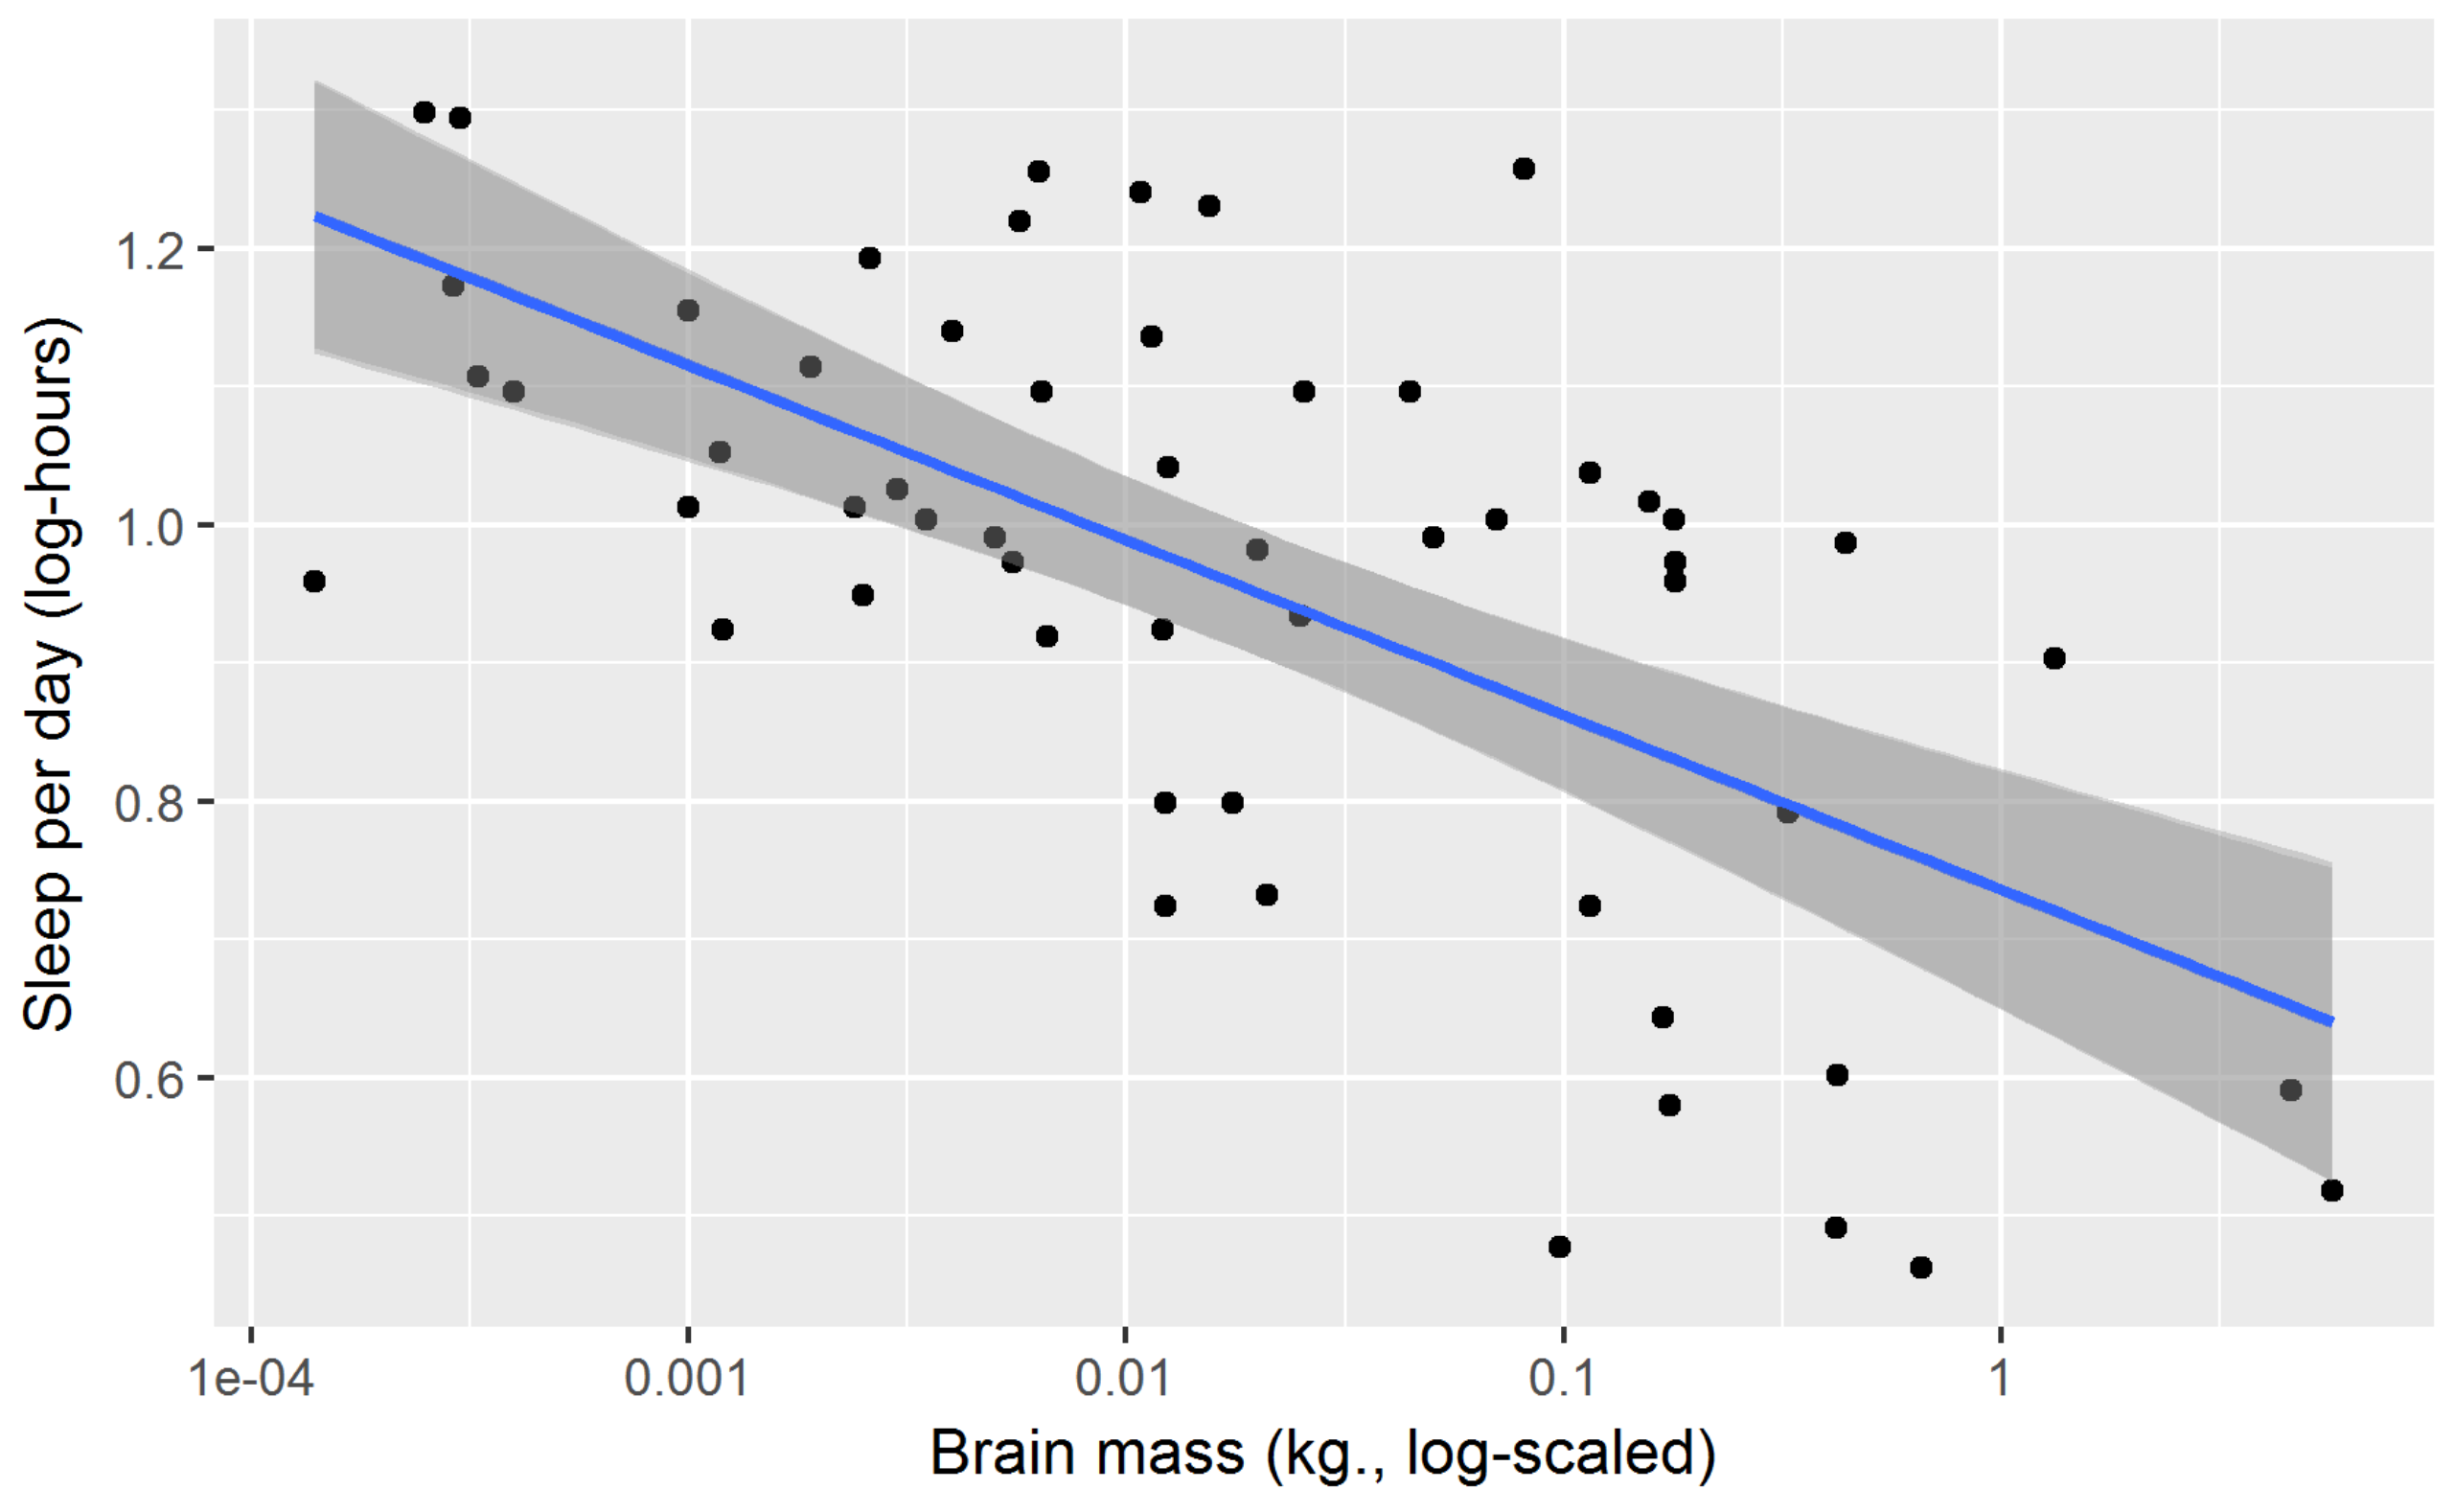
\includegraphics[scale=0.2]{PI-reg2}
	\end{center}
	
\end{frame}


\end{document}